\section{Data}

\subsection{Data sources and collection}
We leverage the following data sources in this analysis:
\begin{table*}[t]
\begin{center}
  \begin{tabular}{| p{3cm} | p{5cm} | p{6cm} |}
    \hline
    Variables &  Description & Source \\ \hline
    Forest Cover& NASA Long Term Data Record measurements of vegetative cover & \url{http://ltdr.nascom.nasa.gov/cgi-bin/ltdr/ltdrPage.cgi }\\ \hline
    World Bank Project Locations & Double-blind geocoded information on the geographic location of each World Bank project & \url{http://aiddata.org/level1/geocoded/worldbank} \\ \hline
    Distance to Rivers & The calculated average distance to all rivers & \url{http://hydrosheds.cr.usgs.gov/index.php} \\ \hline
    Distance to Commercial Rivers & Calculated average distance to all commercial rivers & \url{http://hydrosheds.cr.usgs.gov/index.php}  \\ \hline
    Distance to Roads &  Distance to nearest road & \url{http://sedac.ciesin.columbia.edu/data/set/groads-global-roads-open-access-v1}\\ \hline
    Elevation & Elevation data measured from the Shuttle Radar Topography Mission & \url{http://www2.jpl.nasa.gov/srtm/}\\ \hline
    Slope&  Slope data calculated based on the Shuttle Radar Topography Mission & \url{http://www2.jpl.nasa.gov/srtm/}\\ \hline
    Accessibility to Urban Areas & European Commission Joint Research Centre estimation of urban travel times. & \url{http://forobs.jrc.ec.europa.eu/products/gam/download.php}\\ \hline
    Population Density & Center for International Earth Science estimation of population density, derived from Nighttime Lights & \url{http://sedac.ciesin.columbia.edu/data/collection/gpw-v3}  \\ \hline
    Air Temperature & University of Delaware Long term, global temperature data interpolated from weather station measurements. &\url{http://climate.geog.udel.edu/~climate/ }\\ \hline
    Precipitation & University of Delaware Long term, global precipitation data interpolated from weather station measurements.& \url{http://climate.geog.udel.edu/~climate/}\\ 
    \hline
    
  \end{tabular}
  \caption{Covariates of the data sets for World Bank projects}
  \label{table:data}
\end{center}
\end{table*}
    
\subsection{Data pre-processing}
  This analysis uses three key types of data: satellite data to measure vegetation, data on the geospatial locations of World Bank projects, and covariate datasets (the sources of which are detailed above). 
Our primary variable of interest is the fluctuation of vegetation proximate to World Bank projects, which is derived from long-term satellite data (NASA 2015). 
There are many different approaches to using satellite data to approximate vegetation on a global scale, and satellites have been taking imagery that can be used for this purpose for over three decades.  
Of these approaches, the most frequently used is the Normalized Difference Vegetation Index (NDVI).  The NDVI is a metric that has been used since the early 1970s, and is one of the simplest and most frequently used approaches to approximating vegetative biomass.  
NDVI measures the relative absorption and reflectance of red and near-infrared light from plants to quantify vegetation on a scale of -1 to 1, with vegetated areas falling between ~0.2 and 1. 
The reflectance by chlorophyll is correlated with plant health, and multiple studies have illustrated that it is generally also correlated with plant biomass. 
In other words, healthy vegetation and high plant biomass tend to result in high NDVI values (Dunbar 2009).  
Using NDVI as an outcome measure has a number of other benefits, including the long and consistent time periods for which it has been calculated.  
While the NDVI does have a number of challenges - including a propensity to saturate over densely vegetated regions, the potential for atmospheric noise (including clouds) to incorrectly offset values, and reflectances from bright soils providing misleading estimates - the popularity of this measurement has led to a number of improvements over time to offset many of these errors.  
This is especially true of measurements from longer-term satellite records, such as those used in this analysis, produced from the MODIS and AVHRR satellite platforms (NASA 2015).
\par
The second primary dataset used in this analysis measures where - geographically - World Bank projects were located.  This dataset was produced by AidData (2016), relying on a double-blind coding system where two experts employ a defined hierarchy of geographic terms and independently assign uniform latitude and longitude coordinates, precision codes, and standardized place names to each geographic feature. If the two code rounds disagree, the project is moved into an arbitration round where a geocoding project manager reconciles the codes to assign a master set of geocodes for all of the locations described in the available project documentation. This approach also captures geographic information at several levels?coordinate, city, and administrative divisions?for each location, thereby allowing the data to be visualized and analyzed in different ways depending upon the geographic unit of interest. Once geographic features are assigned coordinates, coders specify a precision code that varies from 1 (exact point) to 9 (national-level project or program).
AidData performs many procedures to ensure data quality, including de-duplication of projects and locations, correcting logical inconsistencies (e.g. making sure project start and end dates are in proper order), finding and correcting field and data type mismatches, correcting and aligning geocodes and project locations within country and administrative boundaries, validating place names and correcting gazetteer inconsistencies, deflating financial values to constant dollars across projects and years (where appropriate), strict version control of intermediate and draft data products, semantic versioning to delineate major and minor versions of various geocoded datasets, and final review by a multidisciplinary working group. 
\par
In addition to the project name, the World Bank provided information on donors and amounts of funding for each project.
For a subset of project, there is data on the performance evaluation of projects for evaluating effectiveness of staff. 
We also learnt that a single project rarely resides on a single location. It typically spreads out over a number of n locations with typical values of $n=2$ but ranging up to $n=10$.

\subsection{Data characteristics}
For variables listed in the Table \ref{table:data} excluding the geographic location, population density and NDVI, we have minimum, maximum, and average values for each year between 1992 and 2012. For NDVI and population density, we only have a time series with average annual values. The project's geographic location is assumed constant. While annual values for covariates such as elevation and slope are typically constant over time, for others we expect to see change over time, in particular those in response to economic development such as distance to roads, accessibility to urban areas and population density. Air temperature and precipitation describe environmental conditions that may change subject to long-term trends due to a change in climate, subject to multi-year seasonal effects due to the El Nino Southern Oscillation, and subject to local or regional environmental changes, e.g. a massive deforestation. For lack of space, we only describe some characteristics of NDVI data.
Figure \ref{fig:ndvi} a) shows average annual NDVI values of all project locations for each year since 1982. The mean values are non-negative for all projects over all years and typical values are around 0.2 which is a lower bound for areas with vegetation.
For each project location, the average annual NDVI values give a time series for which we can do a linear regression fitting to estimate the slope of an underlying trend. Figure \ref{fig:ndvi} b) shows the distributions of slope values for a time series of NDVI values that starts in 1982 and ends with the year before the project starts. We see that regardless of the year the projects start, more than 75\% of all projects face a starting situation where NDVI values are slightly on the rise.

\begin{itemize}
%\item provide an overview of the total number of covariates and their characteristics. As in table \ref{table:data}, the main covariates are in the table, for temperature, precipataion, they both have data for 20 years including maximum, minimum,average value of each year, also the NDVI values and avg light percentage value for 20 years but only contains average value. There are also some other covariates that not in the table, such as project name, the donors, the fund of the projects, we refer people who interest in the data to aiddata website for details. 
%\item Forest cover (= NDVI?): time series. As this is an important variable, can we get a box plot with mean values and slope values for all projects? 
\item for covariates, we should provide some outline about type (categorical, ordinal,numerical), ranges of values, and if some normalization is applied. If data gives a time series, its granularity (time and space), concerns about precision
(no space for too much details about the data, we can refer them to aiddata website for details)
\item set of world bank projects covers a broad range of topics and individual projects do not necessarily directly target deforestation. We want to recognize projects that show an impact on forest cover, be it positive or negative. (too many projects to check, can only guess from the title)
\item discuss projects and project locations: a project can take place at more than one geographic location.( The data contains projects that have between 1 and 10 locations. )  One project may contains sub projects in different locations from one to hundreds.  This raises the question on how to aggregate average treatment effects across a set of project locations into a single value for the overall project.
\end{itemize}


\begin{figure}
	\subfloat[]{  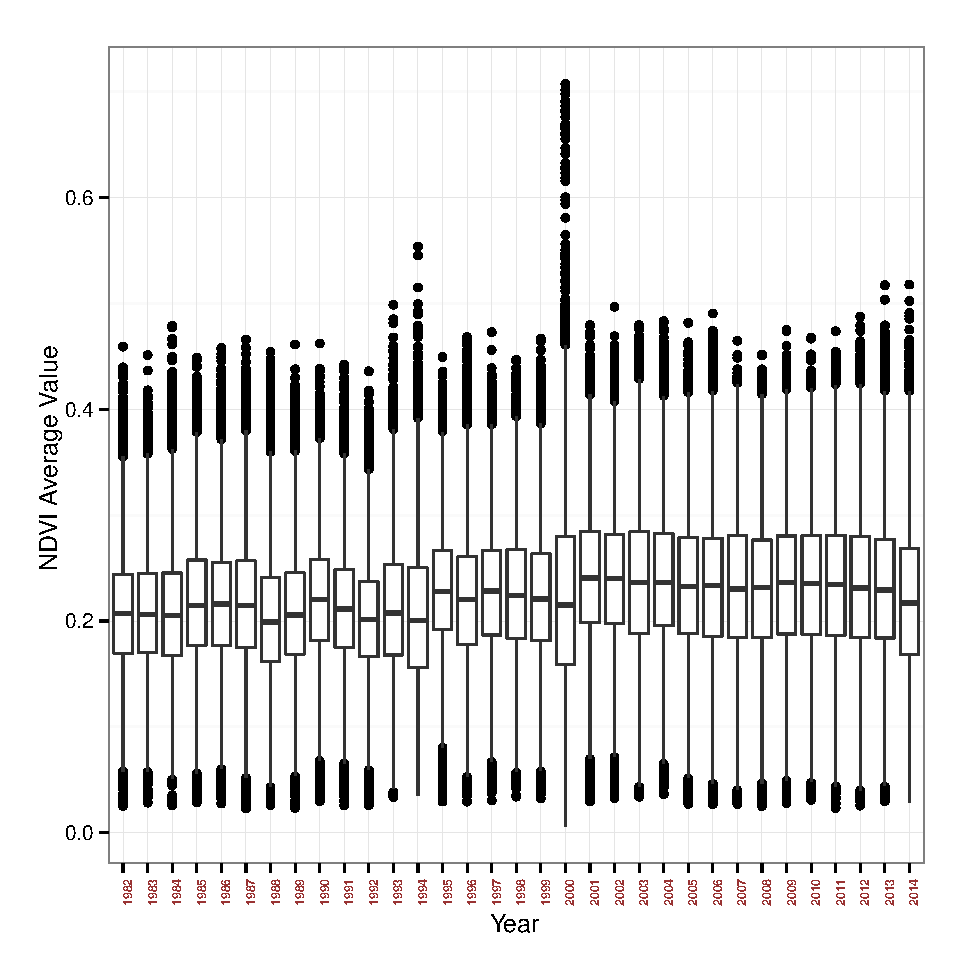
\includegraphics[width=0.5\textwidth]{figs/ndvi.eps}}	
	\subfloat[]{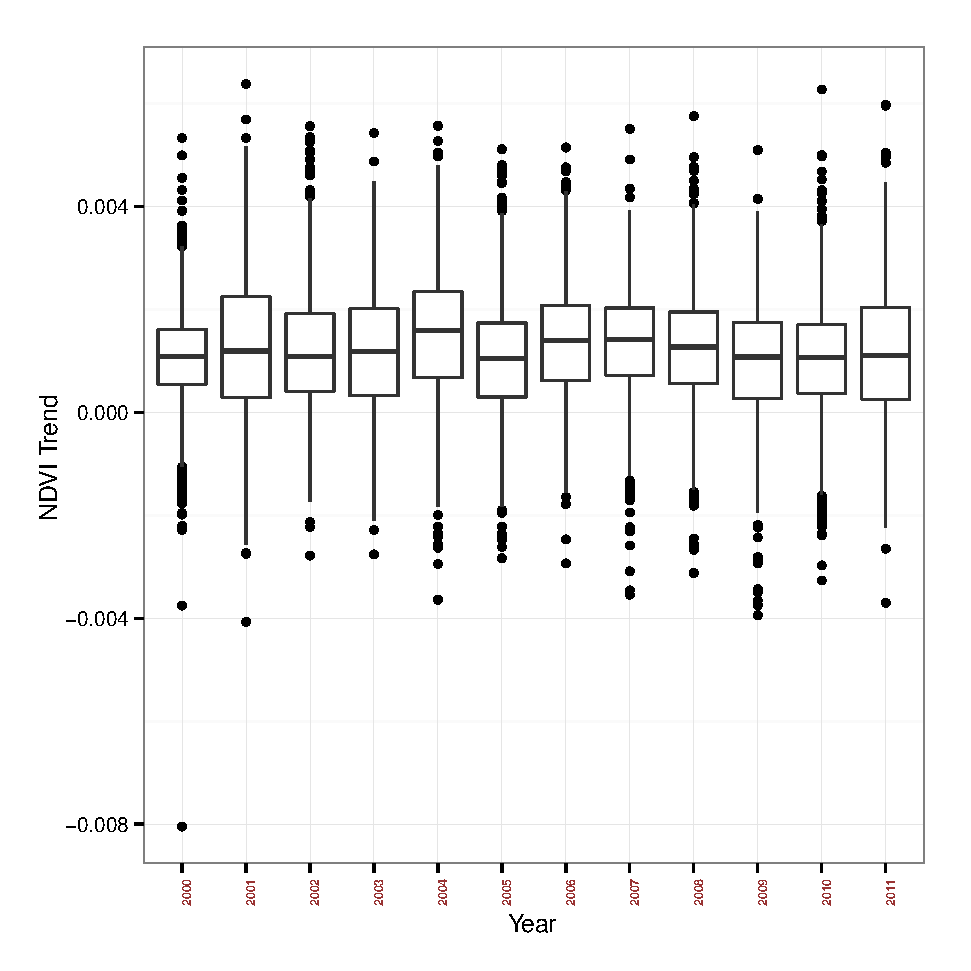
\includegraphics[width=0.5\textwidth]{figs/ndvitrend.eps}}	
	\caption{NDVI features of all the projects} \label{fig:ndvi}
\end{figure}


\subsection{Data interpretation for the context of measuring heterogenous treatment effects}
CT and TOT methods expect a separation of the data set into treated and untreated cases.
A treatment in our setting is of course the fact that a project takes place. As our data set only contains project data, we make the assumption that the observed treatment effect should positively correlate with the amount of funding, i.e. huge amounts of funding are expected to have a bigger effect than small amounts of funding. In this way, we assign $W_i=1$ if a project's funding exceeds a fixed threshold of \$ xxx.
The data set contains 1168 projects in 16415 locations that were performed between 2001 and 2012. Many covariates are described with time series data which leads to the question on how to compare projects that started in different years. One possibility is to retain absolute values for points in time, i.e. precipitation in 2002, which has the benefit to keep numerical comparisons of actual precipitation values across projects meaningful (if that year was a draught season in a large region) but creates the difficulty that projects have a variable set of features as we can not include covariates for the time after the project begins. Another possibility is to use time stamps relative to the project start, i.e. have values for $1,2,3,...,k$ years before the project starts. The benefit is that all units can share the same set of covariates (after some truncation), but for example the comparison of values for precipitation 3 years before a project stars across some projects may ignore hidden global constraints. This effect gets more pronounced if one compares the outcome, the NDVI values for years following the project, in the computation of the response $Y$. A further option is to aggregate time series data into fewer features, e.g. to represent it by a linear model and use intercept and slope.
This incorporates further assumptions and shares the same issues mentioned before for relative time stamps. 
In order to avoid this issue, we decided to focus on a subset of projects that all started in the same year. We selected the year 2004.
As a single project typically takes place at several project locations, we decided to consider each project location as an individual unit. 
This means, the overall data set of 114 projects that started in 2004 at a total of 1628 project locations gives $n=1628$ units.
For the feature vector, we include longitude and latitude of the geolocation and time series data for other variables till the beginning of a project. As CT and TOT methods tolerate large numbers of covariates but can not perform functions such as average over a set of features, we decided to include annual values for time series data plus estimates of average and slope (as for example shown for NDVI in Fig. \ref{fig:ndvi}). The idea is to recognize if the analysis method has a preference for a particular year or for average or slope.
The total length of the feature vector is $d=XXX$. All covariates are numerical and their values are taken as is and not normalized. 
%The response $Y_i$ of a project location $i$ is the slope of a linear regression that we perform on annual average NDVI values for the years 2004 till 2010, i.e. six years from the beginning of the project.
Let $ndvi_i(92,03)$ denote the average of NDVI values observed for project location $i$ over the years from 1992 to 2003 before the project starts. Let $ndvi_i(05,12)$ describe the corresponding value for the eight years after the project starts.
%The response $Y_i = ndvi_i(05,12)-ndvi_i(92,03)$ of a project location $i$ is the difference of average NDVI values over six year periods before and after the beginning of the project.
The response $Y_i = ndvi_i(05,12)-ndvi_i(92,03)$ is the difference of the two averages.
In order to calculate $Y^\ast$ for $Y$, we need to obtain the propensity score $e(x)$, which describes the expected value for treatment $W_i$ for a given feature vector $x$. Note that the propensity score for each unit is calculated in a preprocessing step that is independent from the applied CT or TOT method. 

\begin{itemize}
\item describe how we calculate propensity scores: We use linear model to calculate the pscore. 
\end{itemize}
 



%\begin{itemize}
%\item general idea is to separate data into treated and untreated cases, there is no particular notion of time. For each entity (treated or untreated), a set of covariates are provided.
%\item in our case: we decided to interpret the project start as the treatment and the change in forest cover (average?, slope?) as the treatment effect. We use average before 1992-2003 for ndvi and 2005-2012.
%\item as we only have data for locations were a project takes place, we consider small scale projects with small amounts of funding as untreated cases (???)
%\item We decided for time series data: split into two parts, before and after project start. We only take covariates for data before project starts into account for selecting variables in the random forest construction. We use data after the project starts to compute treatment effects. Rationale: covariates with data after treatment may be correlated with the outcome which would corrupt the calculation of average treatment effects (?).
%\item Since large scale correlations and changes beyond the reach of the project such as the beginning or ending of a draught period over several years may by hiding within time series data, we decided to compare projects that all started in the same year in order to have level playing field for projects in the same geographic region.
%\end{itemize}
%
%\subsection{Calculation of Propensity Scores}
%\begin{itemize}
%\item describe how we calculate propensity scores before we feed the data into a random forest. We use linear model to calculate the pscore. 
%\end{itemize}


